\lab{Application}{K-Nearest Neighbors}{K-Nearest Neighbors}
\label{Ch:KNN}

\objective{Implement a K-Nearest Neighbors classification algorithm using the Nearest Neighbor search from the previous section}

\section*{Classification}

A common problem is correctly classifying data.  Suppose that you have a ten marbles.  Suppose further that five of your marbles are blue with a green stripe and the other five are red with a purple stripe.  If your friend gave you an eleventh marble that was blue with a brown stripe, which group would you put it in?  Probably you would include it with the other blue marbles.  What if the marble that your friend gave you was blue with a purple stripe?  This marble shares characteristics with both groups.  Where you end up grouping it will depend on which characteristics are most important to you.

This is the intuitive classfication problem.  If we have data that is grouped into some sets for us, what set do we put new data into?  Classification has myriad and sundry applications.  In this lab we will use it in an optical character recognition application.

\section*{Nearest Neighbor Classification}

We now more formally describe the classification problem and explain the nearest neighbor classification algorithm.  Suppose that we have a collection of vectors $\{x_1, ..., x_m\}$ in $\R^n$ with corresponding labels $\{l_1, ..., l_k\}$ describing to which group each datum belongs.  This collection of vectors and labels is called our training set.  Each entry of a vector is called a feature, and $n$ is the size of our feature set.  For example, consider the following vectors in $\R^3$

\begin{center}
\begin{tabular}{cc}
$(2,0,0)$ & $1$ \\
$(3,0,0)$ & $1$ \\
$(0,3,0)$ & $2$ \\
$(0,2,0)$ & $2$ \\
$(\frac{1}{10},2,0)$ & $2$ \\
$(0,0,4)$ & $3$ \\
$(0,0,7)$ & $3$ \\
\end{tabular}
\end{center}

If we also have a metric on our space, we may determine the distance between all of these points.  If we are given a new datum and we wish to decide which of the three groups to include it in, one option is to choose the group to which it's closest neighbor belongs.  Let us use the euclidean metric to classify $(0,0,5)$ against our training set.  We see that the distance from $(0,0,5)$ and $(0,0,4)$ is only $1$, while the distance to the remaining points is at least $2$.  The label of $(0,0,4)$ is $3$, and so we assign $(0,0,5)$ the same label.

Now, what if we wished to classify $(\frac{5}{2},\frac{5}{2},0)$?  This presents a problem since this point is equidistant from the points in label $1$ and label $2$.  In such a case it is up to the programmer to decide how to break the tie.

One case we need to consider is when the data that we are using in our search are on different scales. For example, suppose we wished to classify people applying for a loan at a bank as `risky' or `safe.'  Further suppose that we know their age, education level, current debt, and how many credit cards they have.  We could encode their education level as integers between $0$ and $4$.

Suppose that Bob is 30 years old, well educated, has a debt of \$5000, and 3 credit cards.  Let's say that James is 18 years old, barely out of high school, \$5000 dollars in debt, and own 4 credit cards.  If we were to use the Euclidean metric $d$ to measure how close Bob is to James, we would get a distance of
\[
d((30,4,5000,3),(18,0,5000,4)) = 12^2 + 4^2 + 1^2 = 161.
\]

However, if Alice is well 29 years old, well educated, has a debt of \$4900, and 3 credit cards, then her distance from Bob is
\[
d((30,4,5000,3),(29,4,4900,3)) = 1^2 + 100^2 = 100001.
\]

Is James closer to Bob than Alice?  Most Banks would say no.  In order to classify these individuals better, we need to measure distance differently. There are two different ways to handle this. The first is we could scale the data before inputting it into our algorithm. In our previous example we could divide age by 100, education by 4, debt by 1000 and credit cards by 10 and then preform a nearest neighbor search on Bob. Then the distance from Bob to James is 
\[
d((\frac{30}{100},\frac{4}{4},\frac{5000}{1000},\frac{3}{10}),(\frac{18}{100},\frac{0}{4},\frac{5000}{1000},\frac{4}{10})) = .12^2 + 1^2 + .1^2 = 1.0244.
\]
while the distace from Alice to Bob is
\[
d((\frac{30}{100},\frac{4}{4},\frac{5000}{1000},\frac{3}{10}),(\frac{29}{100},\frac{4}{4},\frac{4900}{1000},\frac{3}{10})) = .1^2 + .01^2 = 0.0101.
\]
So now Bob is closer to Alice.

\begin{problem}

Write a function that takes in data points and the a vector that is used to be the scale. The function outputs the scaled data points. So if we were using it for our baking example it would take in the array representing the data Alice, Bob and James (where each person is a row) and the vector $[100,4,1000,10]$ and output the scaled data of Alice, Bob and James.

\end{problem}

Another alternative is changing the metric we used to measure distance with. In both the examples above we used our algorithm to measure distance used the Euclidean metric. Suppose one piece of data we had was color where 1 was red, 2 was violet, 3 was blue, 4 was green, 5 was yellow, 6 was orange. If we use Euclidean distance green is closer to red than orange is where is reality we want orange to be the same distance from red as violet is. The best solution would be to write your metric function that took this into account. 


\section*{K-Nearest Neighbor Classification}

Often we can improve the accuracy of a classifier by looking other points beside the nearest neighbor.  Instead, we may choose an arbitrary number $k$ and give the point to be classified the majority label in from it's $k$ nearest neighbors. 

There are pitfalls to this approach.  Consider a point that's closest neighbor has the label $0$.  If we only considered the nearest neighbor, then we would be finished.  However, what if the next $10$ nearest neighbors all had the label $1$?  Do you think that we should still classify the point as $0$?  What if the nearest point has a distance of $0.1$ and the next $10$ points have a distance of at least $100$?  The answer to these questions depend on the kind of data we are working with and the metric that we choose.  One should ensure to consider how to treat situations like this when working on classification algorithms.


The sklearn library has neighbors module that has a KNeighborsClassifier
\begin{lstlisting}
from sklearn import neighbors
nbrs = neighbors.KNeighborsClassifier(n_neighbors=8 ,weights = 'distance' ,p=2)
\end{lstlisting}

The \li{neighbors.KNeighborsClassifier} sets up your knearestnieghbor algorithm. \li{n_neighbors} how many neighbors you would like to find  and \li{weights} is how you would like to weight the neighbors you have to make the classification. weights can be \li{'uniform'}, the majority of the k classifications is what the new value will be classified as, or \li{'distance'}, where it weights the classifications nearer to the point heavier than those far away. The argument \li{p} correpsods to the distance metric. For this lab we will use \li{p=2} which is the Euclidean distance.  

\begin{lstlisting}
nbrs.fit(points, labels)
\end{lstlisting}
Points and labels are your training data. The \li{fit} function makes the \li{nrbs} make a data structure containing those points and labels that is ready to be queried. 

\begin{lstlisting}
nbrs.predict(testpoints)
\end{lstlisting}

Theses are the points you want to classify. The output is the labels that the points correspond to. More information about this package can be found at http://scikit-learn.org/stable/modules/neighbors.html.
\begin{problem}

Get the post office handwritten digit data set. Load with
\begin{lstlisting}
labels,points,testlabels,testpoints=np.load('PostalData.npz').items()
\end{lstlisting}
This contains a training set and a test set. When you load the first entry is a name. So \li{points[1]} and \li{labels[1]} are the actual points and labels you want to use. Each point is a  image that is $28 \times 28$ matrix of pixels that has been flattened. The corresponding label indicates which number was written.  Try classifying the testpoints with \li{n_neighbors} being 4 and then 10 and \li{weights} being \li{'uniform'}, and then \li{'distance'}. Then do the classfication with \li{n_neighbors} being 1. For each one return a report indicating how your classifier performs in terms of misclassifications as a percentange (testlabels are the labels that correspond to the testpoints). Which one does the best?

A similar classification process is used by the United States Postal Service to automatically determine the zip code to send a letter to.

\end{problem}

\begin{figure}[h]
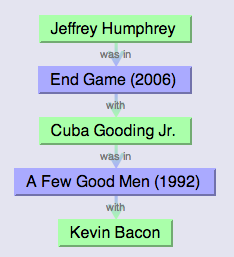
\includegraphics[scale = 4]{Example.png}
\caption{An example of the number 6 taken from the data set}
\end{figure}




















































